\documentclass[en]{article}
\usepackage[left=2.2cm,right=2.2cm,top=2.5cm,bottom=2.5cm]{geometry}
\usepackage[utf8]{inputenc}
\usepackage{minted}
\usepackage{booktabs}
\usepackage{commath}
\usepackage{float}
\usepackage{mathtools}
\usepackage{amsthm}
\usepackage{parskip}


\usepackage[binary-units=true]{siunitx}

\newcommand{\py}[1]{\mintinline{python}{#1}}

\title{Artificial Intelligence (\texttt{LINGI2261}) \\ Assignment 2 --- Group 13}
\author{Martin Braquet, Gilles Peiffer}

\begin{document}

\maketitle

\section{Alpha-Beta search}

\subsection{MiniMax algorithm}

\begin{figure}[H]
 \centering
 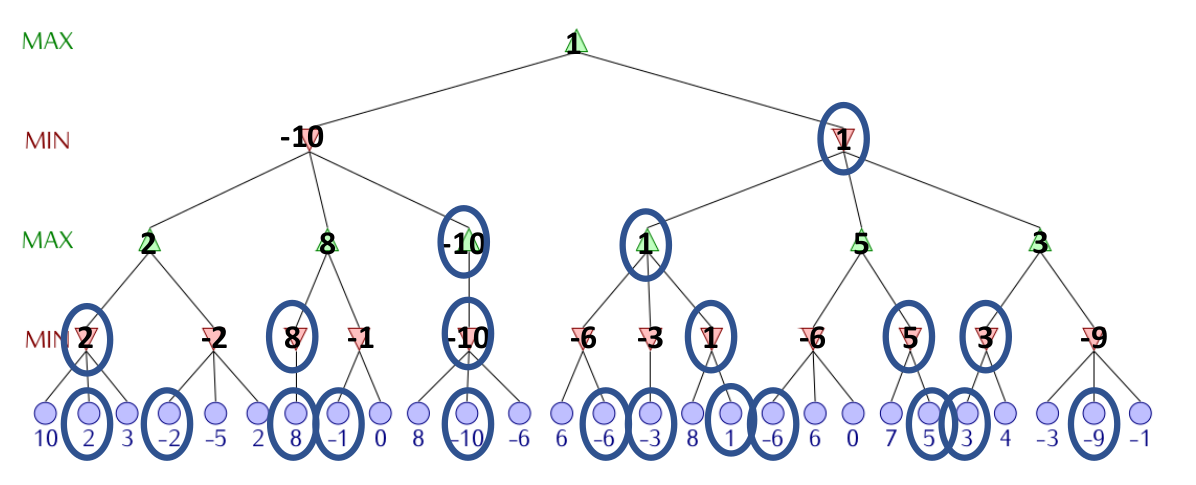
\includegraphics[width=\textwidth]{MiniMax.png}
 \caption{Minimax algorithm}
 \label{fig:minimax}
\end{figure}


\subsection{Alpha-Beta algorithm (left to right)}

\begin{figure}[H]
 \centering
 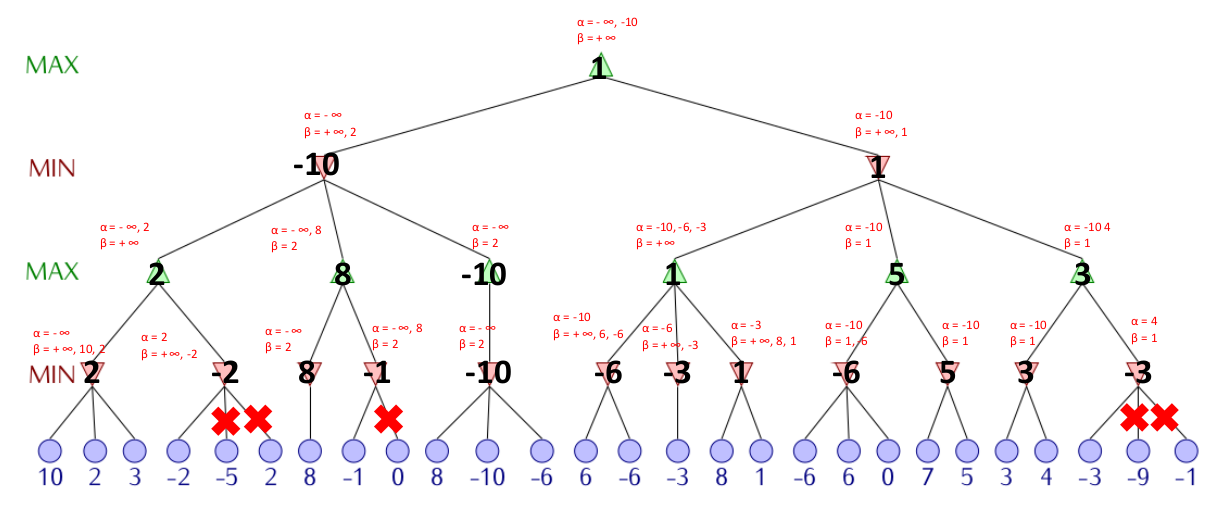
\includegraphics[width=\textwidth]{Alphabeta.png}
 \caption{Alpha-Beta algorithm (left to right)}
 \label{fig:alphabeta}
\end{figure}


\subsection{Alpha-Beta algorithm (right to left)}

\begin{figure}[H]
 \centering
 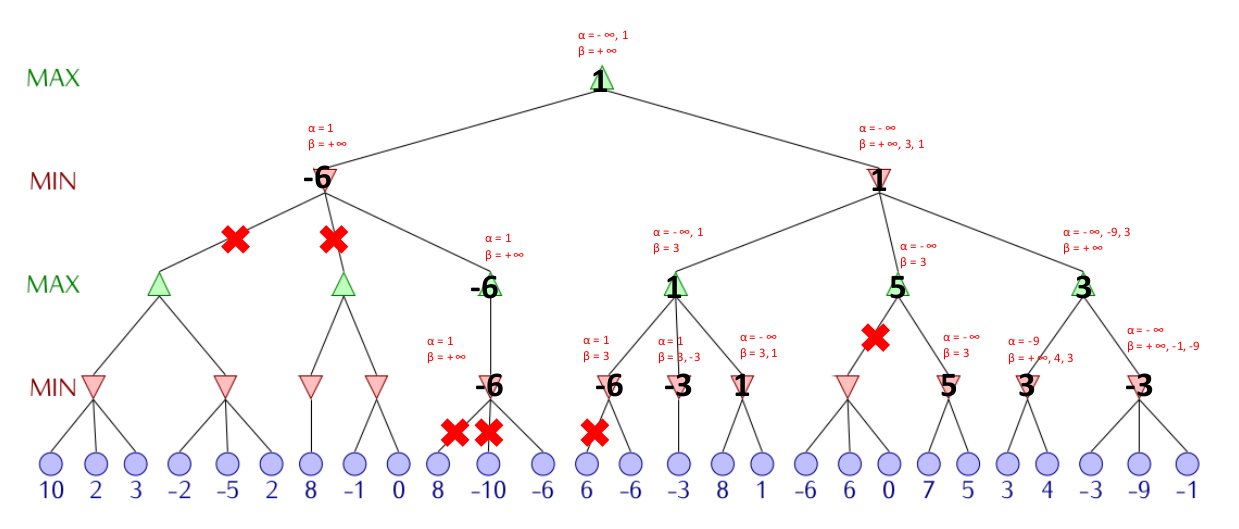
\includegraphics[width=\textwidth]{Alphabeta_reverse.png}
 \caption{Alpha-Beta algorithm (right to left)}
 \label{fig:alphabeta_reverse}
\end{figure}


\subsection{Alpha-Beta algorithm (ordered)}

\begin{figure}[H]
 \centering
 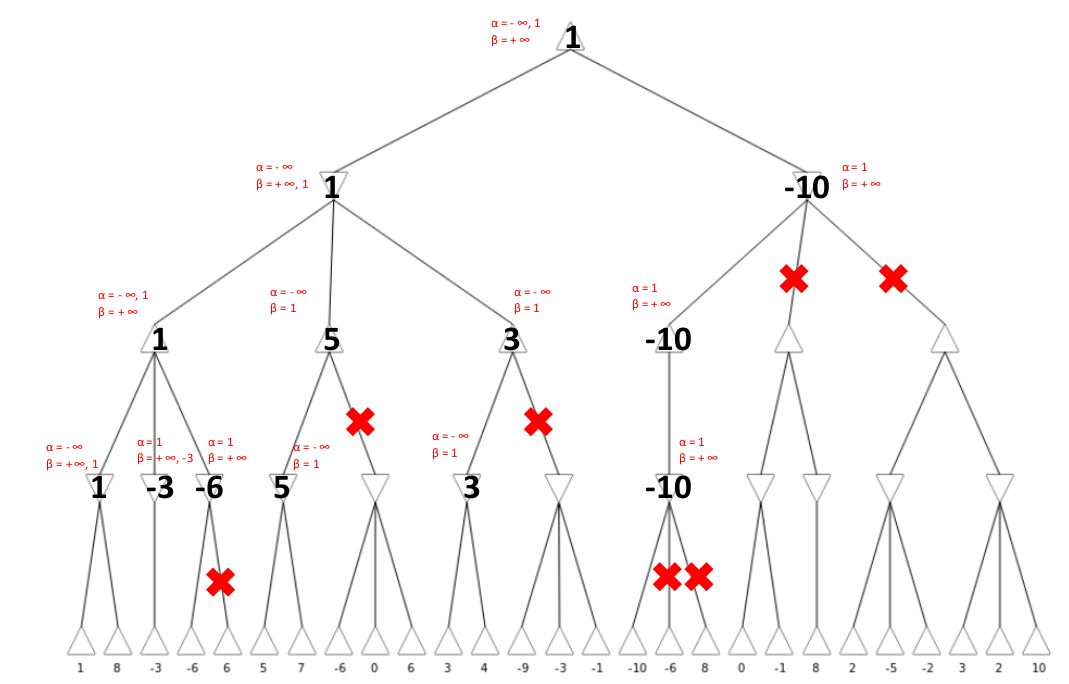
\includegraphics[width=\textwidth]{Alphabeta_ordered.png}
 \caption{Alpha-Beta algorithm}
 \label{fig:alphabeta_ordered}
\end{figure}

\subsection{Alpha-Beta for more than two players}

For more than two players, each node is associated with a tuple giving the value of each player for that state.

Tree pruning is possible if there is an upper bound on the sum of all components of this tuple, and there is a lower bound on the values of each component. We define the sum $S$ as the global upper bound on the sum of all components of the N-tuple, and all components are
assumed to be non-negative. 

The condition \py{v <= alpha} and \py{v >= beta} is now given by \py{Best[Player] >= Bound} where the bound equals the sum $S$ minus the last best node of the upper layer. Indeed, let's take a player 1 from the upper layer which is ensured to get a value of at least $x$ for his layer: $(\ge x, \dots, \dots)$. Then, if player 2 from the lower layer unveils a child with more than $S - x$ for its own value, it will result of a score $(\le x, \ge S - x, \dots)$. Thus, all the remaining children can be dropped since player 1 knows that these children will be chosen by player 2 only if the value of player 1 is less than $x$ \cite{multiplayer}.

\begin{figure}[H]
 \centering
 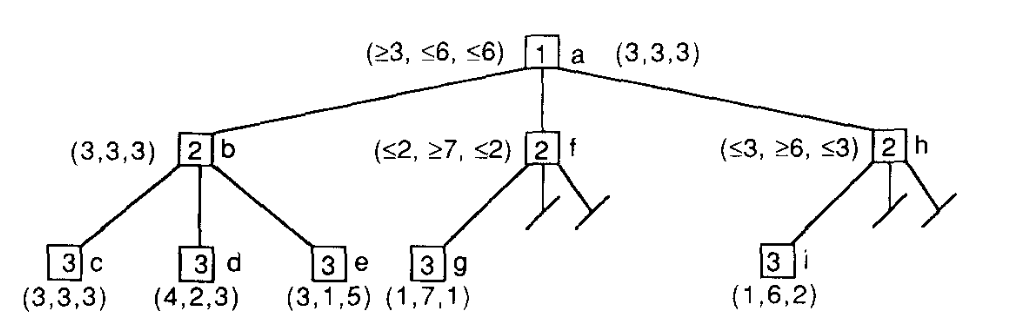
\includegraphics[width=0.7\textwidth]{multiplayer.png}
 \caption{Shallow pruning in three-player game tree \cite{multiplayer}}
 \label{fig:multiplayer}
\end{figure}


\section{Squadro}

\subsection{Comparison of two evaluation functions}

We expect that the new evaluation will work better since it takes into account the opponent, and it will thus prevent the opponent to win for example, by killing his pawns. The old agent is not able to deliberately kill the opponent, consequently decreasing his chances to win.

However, the yellow player still always wins in the four possible starting configurations (which color, who plays first) because he begins with the best paws at the center, progressing by steps of three. The yellow player rapidly puts these paws on the other side, which are then a barrier for the progress of the opponent.
Thus the new basic agent is not good enough to overcome the yellow advantage. 


\bibliographystyle{unsrt}
\bibliography{bib.bib}

\end{document}
